\documentclass[a4paper,11pt]{article}
\pdfoutput=1 
\usepackage{jheppub}
\usepackage{etoolbox}% http://ctan.org/pkg/etoolbox
\makeatletter
\patchcmd{\maketitle}{\@fpheader}{notes package}{}{}
\makeatother

\usepackage[T1]{fontenc}

\usepackage{notespackage}
\usepackage{mytikz}

\usepackage{epigraph}
\setlength{\epigraphwidth}{.7\textwidth}

\usepackage{tikz}
\usetikzlibrary{positioning, calc}
\usetikzlibrary{calc}
\usetikzlibrary{arrows}
\usepackage{tikz-3dplot}
\usepackage{graphicx}
\usepackage{mdwlist}
\usepackage{color}
\newcommand{\blue}[1]{{\color{blue} #1}}
%\usepackage[top=2.5cm,bottom=2.5cm,left=2.5cm,right=2.5cm]{geometry}

\usetikzlibrary{decorations.pathreplacing,decorations.markings}

%specialized tikz settings:
\tikzset{
	%Define standard arrow tip
    >=stealth',
    %Define style for boxes
    punkt/.style={
           rectangle,
           rounded corners,
           draw=black, very thick,
           text width=6.5em,
           minimum height=2em,
           text centered},
    % Define arrow style
    pil/.style={
           ->,
           thick,
           shorten <=2pt,
           shorten >=2pt,},
    % style to apply some styles to each segment of a path
  on each segment/.style={
    decorate,
    decoration={
      show path construction,
      moveto code={},
      lineto code={
        \path [#1]
        (\tikzinputsegmentfirst) -- (\tikzinputsegmentlast);
      },
      curveto code={
        \path [#1] (\tikzinputsegmentfirst)
        .. controls
        (\tikzinputsegmentsupporta) and (\tikzinputsegmentsupportb)
        ..
        (\tikzinputsegmentlast);
      },
      closepath code={
        \path [#1]
        (\tikzinputsegmentfirst) -- (\tikzinputsegmentlast);
      },
    },
  },
  % style to add an arrow in the middle of a path
  mid arrow/.style={postaction={decorate,decoration={
        markings,
        mark=at position .5 with {\arrow[#1]{stealth'}}
      }}}
}

%math environments

\usepackage{epigraph}
\setlength{\epigraphwidth}{.7\textwidth}

\newtheorem{principle}[theorem]{Principle}

\title{The magic square game}
\author[a]{Alex May}
\affiliation[a]{The University of British Columbia}
\emailAdd{may@phas.ubc.ca}

\abstract{The magic square game is an easy to state non-local game which shows a distinct quantum advantage. We describe the game and its optimal quantum and classical strategies.}

\begin{document} 

\maketitle

%%%%%%%%%%%%%%%%%%%%%%%%%%%%%%%%%%%%%%%%%%%%%%%%%%%%%
\section{Introduction and context}
%%%%%%%%%%%%%%%%%%%%%%%%%%%%%%%%%%%%%%%%%%%%%%%%%%%%%

The magic square game is a non-local game with certain attractive features. In particular, it is easy to state and has a quantum strategy that succeeds with unit probability, while a classical strategy succeeds with only $8/9$ probability. We present the game succinctly below. 

The magic square game was developed in the context of quantum foundations, in particular to simplify the understanding of the Kochen-Specker theorem and Bell-type theorems. The system addressed in the game provides a single context wherein both types of theorem may be proven, which illuminates the relationship between the two results. In later notes we will develop these theorems and understand how the magic square game is understood in that context. 

%%%%%%%%%%%%%%%%%%%%%%%%%%%%%%%%%%%%%%%%%%%%%%%%%%%%%
\section{The game}
%%%%%%%%%%%%%%%%%%%%%%%%%%%%%%%%%%%%%%%%%%%%%%%%%%%%%

The rules are:
\begin{enumerate}
    \item Each of Alice and Bob is given a $3\times 3$ grid of squares. They are also told the full set of rules of the game, allowed to decide on a strategy, then are separated. 
    \item After being separated, Alice will be asked to fill in a single row of the grid. Bob will be asked to fill in a single column. They may fill in squares only with $+1$ or $-1$. Call the entries in the square $m_{ij}$. Alice must fill in her row such that the product of the values of the entries is $+1$, Bob should fill in his column such that the product is $-1$. 
    \item Alice's row and Bob's column will meet at one square. Alice and Bob win the game if this entry agrees, and lose if it disagrees. 
\end{enumerate}

After initially being allowed to collaborate and establish a protocol, Alice and Bob are causally separated. The set-up is shown in figure \ref{fig:setup}. 

\begin{figure}
    \centering
    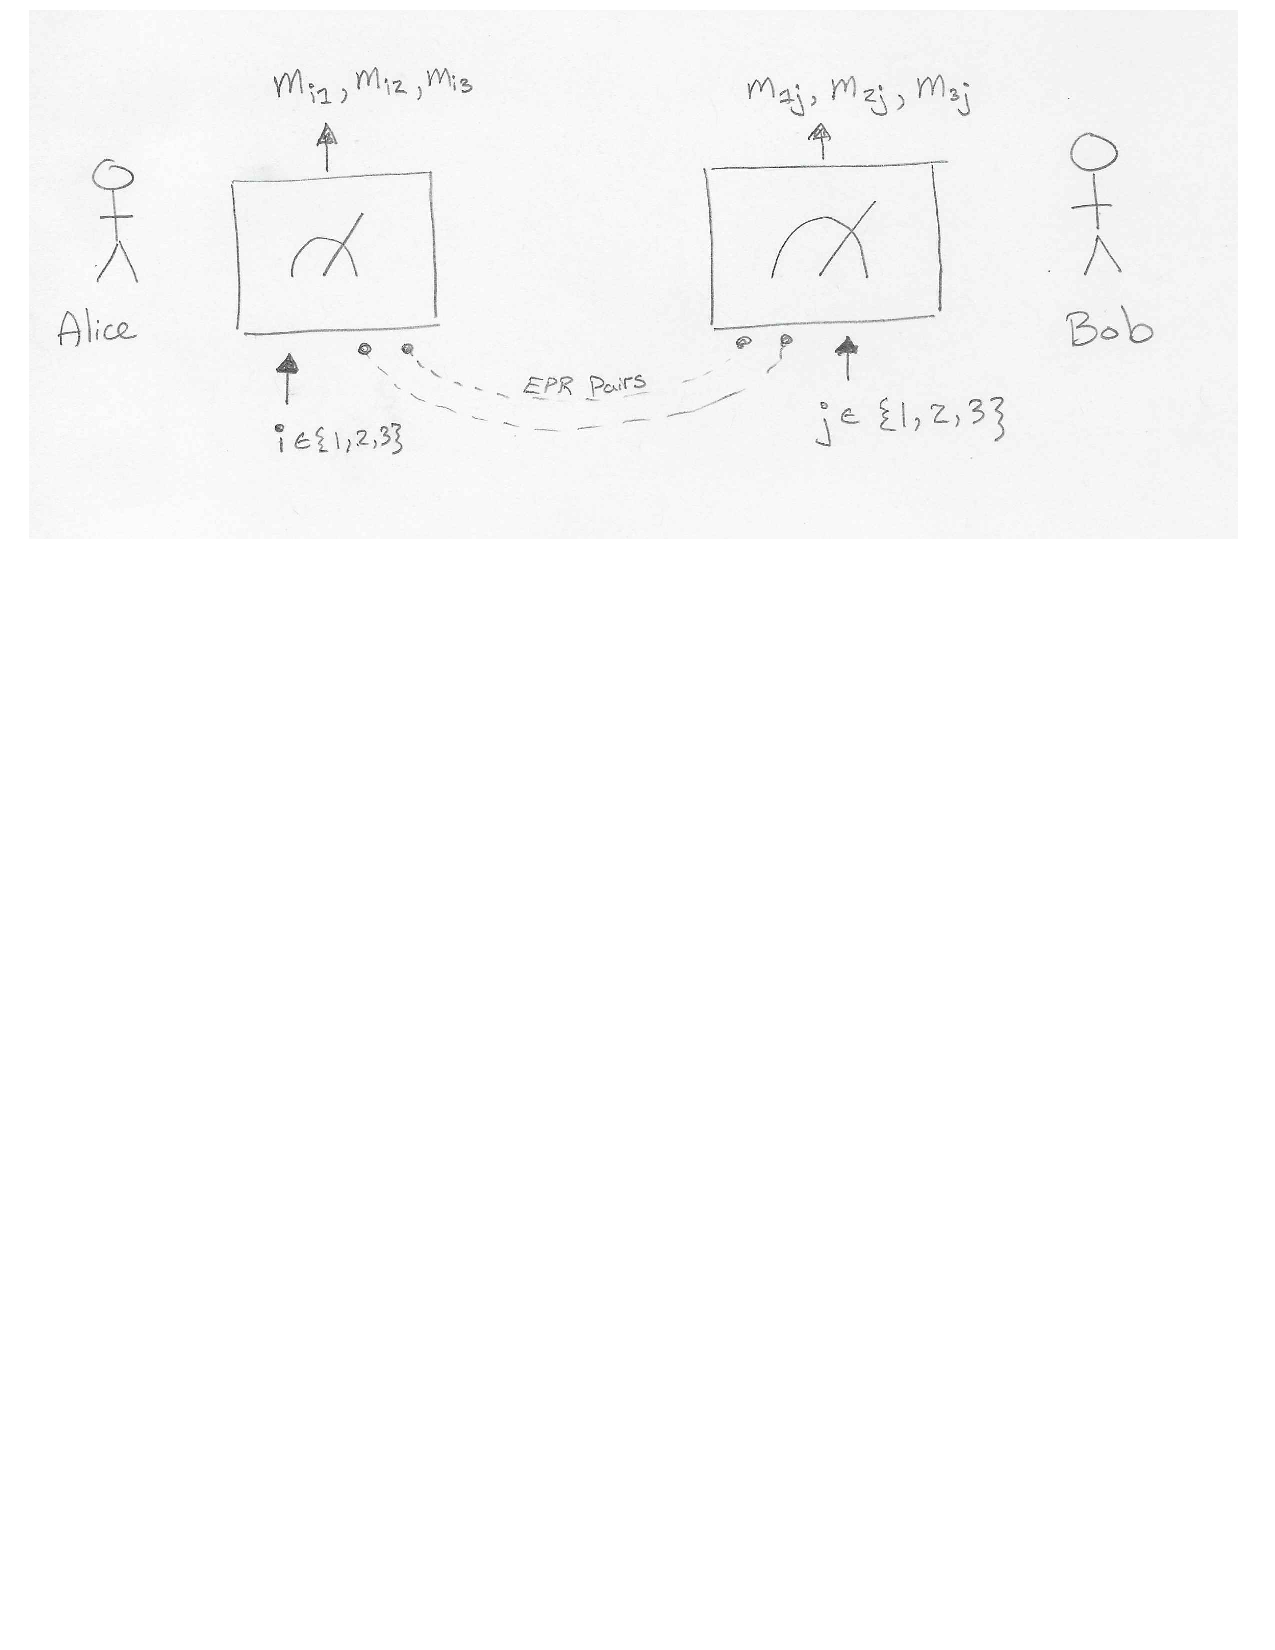
\includegraphics[scale=0.7]{setup.pdf}
    \caption{The basic set-up for the magic square game, depicted in the quantum case. Alice and Bob are spatially separated but share some EPR pairs. Alice is given a specification of a row, while Bob is given a specification of a column. Without communicating, they need to fill in their row or column such that their local constraints are satisfied and their shared entry agrees.}
    \label{fig:setup}
\end{figure}

%%%%%%%%%%%%%%%%%%%%%%%%%%%%%%%%%%%%%%%%%%%%%%%%%%%%%
\subsection{The optimal classical strategy}
%%%%%%%%%%%%%%%%%%%%%%%%%%%%%%%%%%%%%%%%%%%%%%%%%%%%%

Alice and Bob may share classical randomness, along with a set of instructions for what to do given the input specifying the row or column they are to fill in. It is striaghtforward to see however that classical randomness is of no help. This is because their winning probability is
\begin{align}
    p_{win} = \sum_i q_i \, p(\text{win | strategy }\,i)
\end{align}
so that they should choose strategy $i$ with the highest success probability. Thus reduced to deterministic strategies, they should each choose an assignment of values for the squares. Since their goal is to have the intersecting square agree, they do best by choosing the same assignment of values. The problem then is to fill in the 3 by 3 grid with values such that they win the game. 

Recall that Alice and Bob must satisfy constraints on their entries. These are that the rows multiply to $+1$,
\begin{align}
    m_{11}*m_{12}*m_{13} &= 1 \\
    m_{21}*m_{22}*m_{23} &= 1 \\
    m_{31}*m_{32}*m_{33} &= 1
\end{align}
and the columns to $-1$,
\begin{align}
    m_{11}*m_{21}*m_{31} &= -1 \\
    m_{12}*m_{22}*m_{32} &= -1 \\
    m_{13}*m_{23}*m_{33} &= -1 
\end{align}
We can easily see however that these are inconsistent, since if we multiply the  left hand sides of each equation together each $m_{ij}$ appears twice, so this must be $+1$. Meanwhile multiplying the right hand side of each equation together returns $-1$. Consequently no such assignment of values to the $m_{ij}$. This means there is no perfect strategy. 

Instead, Alice and bob must have squares that disagree in one place. This means the strategy will fail whenever that square is the intersection square, which for randomly chosen rows and columns will occur $1$ time out of $9$. The best classical strategy then succeeds with $p=8/9$. 

%%%%%%%%%%%%%%%%%%%%%%%%%%%%%%%%%%%%%%%%%%%%%%%%%%%%%
\subsection{A quantum strategy}
%%%%%%%%%%%%%%%%%%%%%%%%%%%%%%%%%%%%%%%%%%%%%%%%%%%%%

In the quantum case, Alice and Bob's strategy need not involve simply returning values of $m_{ij}$ based on the row and column requests they receive. Instead, they can use their inputs to determine measurement settings, measure some quantum state, then return $m_{ij}$ based on their measurement outcomes. As we will see, the additional resource of holding a shared quantum state allows for perfect completion of the magic square game.

To complete the magic square game with quantum resources, Alice and Bob share two EPR pairs each of which are in the state
\begin{align}
    \ket{\Psi^+}=\frac{1}{\sqrt{2}}(\ket{00}+\ket{11})
\end{align}
Recall that $Z\ket{0}=+\ket{0}$ and $Z\ket{1}=-\ket{1}$. We can also rewrite the above in the eigenbasis of Pauli $X$, 
\begin{align}
    \ket{\Psi^+}=\frac{1}{\sqrt{2}}(\ket{++}+\ket{--})
\end{align}
Alice and Bob will measure their two qubits according to the table shown as figure \ref{fig:magicsquare}. Then, they will output their measurement outcomes as their returned values of $m_{ij}$. 

\begin{figure}
    \centering
    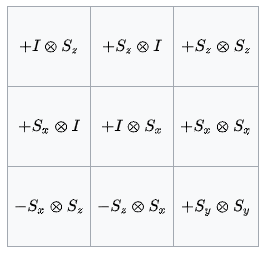
\includegraphics[scale=0.7]{magic_square.png}
    \caption{The ``magic-square''. Notice that the operators in a single row multiply to $+\mathcal{I}\otimes \mathcal{I}$, while in a single column they multiply to $-\mathcal{I}\otimes \mathcal{I}$. Further, the operators within a row or column are mutually commuting.}
    \label{fig:magicsquare}
\end{figure}

Lets understand why this works. First, we can notice that the product of operators along any row is $-I$, while along any column is $+1$. This ensures that Alice and Bobs measurement outcomes satisfy the needed constraints. Next, notice that their measurement outcomes will be perfectly correlated, because of the state we have chosen. Specifically for any EPR pair if both Alice and Bob measure $S_x$, they find the same outcome. Finally notice that Alice and Bob may measure all of the operators in a given row or column, since the operators in any row or column are mutually commuting. From these comments we see that Alice and Bob win the magic square game with a perfect success rate. 

\end{document}
